\chapter{Theoretical Background}
\label{chap:theory}


This chapter deals with the basics of RFID and NFC systems. It explains the principles of communication between the reader and the tag, then introduces the different types of tags and their characteristics, including an explanation of their shortcomings.

\section{Definition of RFID and NFC}

First of all, it is important to explain what RFID and NFC technology actually is. 

\subsection{Definition of RFID}
The main source for this subsection is~\cite{tedjini2005antennas}, unless otherwise specified. RFID stands for "Radio Frequency Identification". It is a wireless sensor technology, which functions on the principle of detecting electromagnetic signals. A standard RFID system configuration consists of three basic elements: 

\begin{itemize}
    \item a tag, which is a small mobile communication circuit embedded on radiating element,
    \item a Base-Station (BS), which is a mobile or fixed transmitter or receiver, and
    \item a database system for the proccessing of the collected data.
\end{itemize}
A schematic of a simplified BS---tag communication protocol is depicted in Figure~\ref{fig:simplified-bs-tag-protocol}.

\begin{figure}[ht]
  \centering
  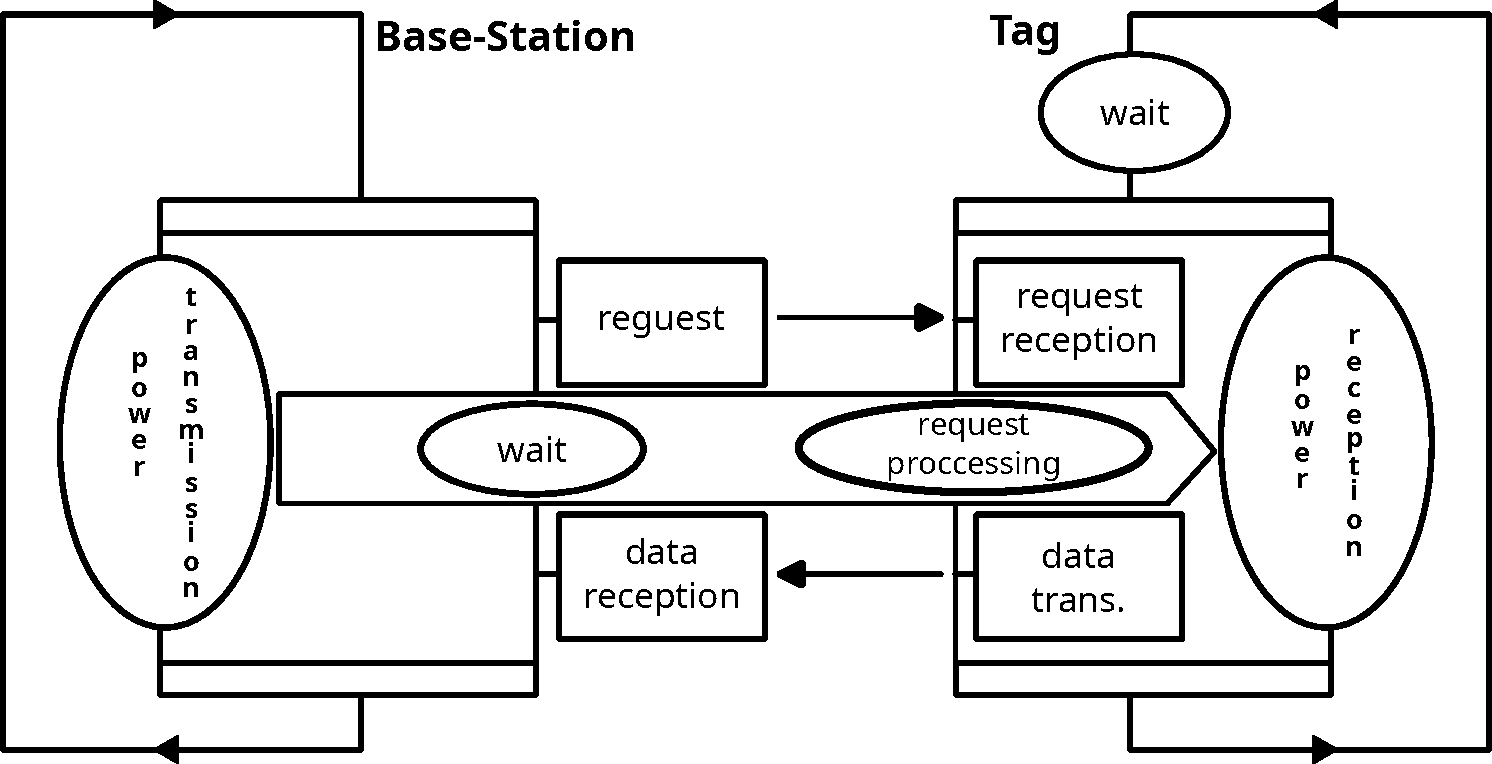
\includegraphics[width=\textwidth]{text/comm_prot.pdf} % or example.eps, depending on the format you converted to
  \caption[A simplified BS---tag communication protocol.]{~A simplified BS---tag communication protocol. Taken from~\cite{tedjini2005antennas}, redrawn by the author.}
  \label{fig:simplified-bs-tag-protocol}
\end{figure} 


RFID tags can be distinguished by the frequencies in which they operate:

\begin{itemize}
    \item low frequency (LF), corresponding to 125 kHz and 134.2 kHz.
    \item high frequency (HF), corresponding to 13.56 MHz, 
    \item ultra-high frequency (UHF), corresponding to 869 MHz, 915 MHz and 950 MHz, and
    \item microwave, corresponding to 2.45 GHz and 5.8 GHz.
\end{itemize}

LF and HF tags are widely produced in the world and used in industries such as security, access control or animal identification. Their limitation is their range, which is less than one meter. However, this is compensated by the fact that there are many affordable and reliable solutions in these frequencies that enable many applications. For needs where greater range is essential, UHF and microwave bands are used --- here the standard reading distance is greater than 3 meters. In the practical part of this thesis we will focus only on LF and HF tags, because these types are used in security and access control systems.

Furthermore, according to their application, RFID tags can be distinguished into active and passive tags. The passive ones are powered by magnetic induction generated by the BS and thus do not need a battery. From now on, in this paper we will restrict ourselves to tags that are passive.


The tag itself is composed of a chip and an antenna, where the antenna has three main functions:

\begin{itemize}
    \item to power the integrated circuit in the tag. The signal sent by the BS is a fixed frequency electromagnetic wave, generating a voltage in the tag circuit;
    \item to receive modulated signal from BS. This signal is a request that must be processed by the tag;
    \item to send the information requested by the BS.
\end{itemize}

\subsection{Definition of NFC}

NFC could be considered a subset of the RFID technology. The NFC communication range is limited to few centimeters and the NFC operates only on 13.56 MHz frequency. While RFID is capable of one-way communication only, the NFC is capable of two-way communication, meaning that the NFC tag can act as both the reader and the tag. RFID technology has anti-collision algorithms that enable scanning of multiple RFID tags at once, while only one NFC tag  can be scanned at a time.~\cite{rfidnfcdifference}


% an antenna or coil, a transceiver, which is equipped with a decoder, and a transponder (RF tag) programmed with unique data. Tag activation and subsequent data transmission are facilitated by the transmission of radio signals from the antenna. Communication between the tag and the transceiver is established via the antennas, while the transceiver controls the data acquisition. The reader, customizable as a handheld or permanently installed, transmits radio waves covering a distance of up to 100 feet, depending on output power and frequency. When the RFID tag is in the electromagnetic field generated by the antenna, it responds to the reader's activation signal. The reader then decrypts the data stored in the tag's integrated circuit, allowing it to be transmitted to any computer system for further processing.


\section{International Standards}

A large number of products and standards fall under RFID and NFC. RFID technology as we know it today began to develop in the 1980s. The International Organization for Standardization (ISO), as well as the International Electrotechnical Commission (IEC), played a fundamental role in the creation of standards. Today's largest manufacturers of RFID chips and equipment include NXP Semiconductors of the Netherlands and Alien Technology of the USA.~\cite{masyuk2019information}

The different sectors of RFID technology, their specifications or applications can be read in Figure~\ref{fig:rfid-graph}.


\begin{figure}[ht]
  \centering
  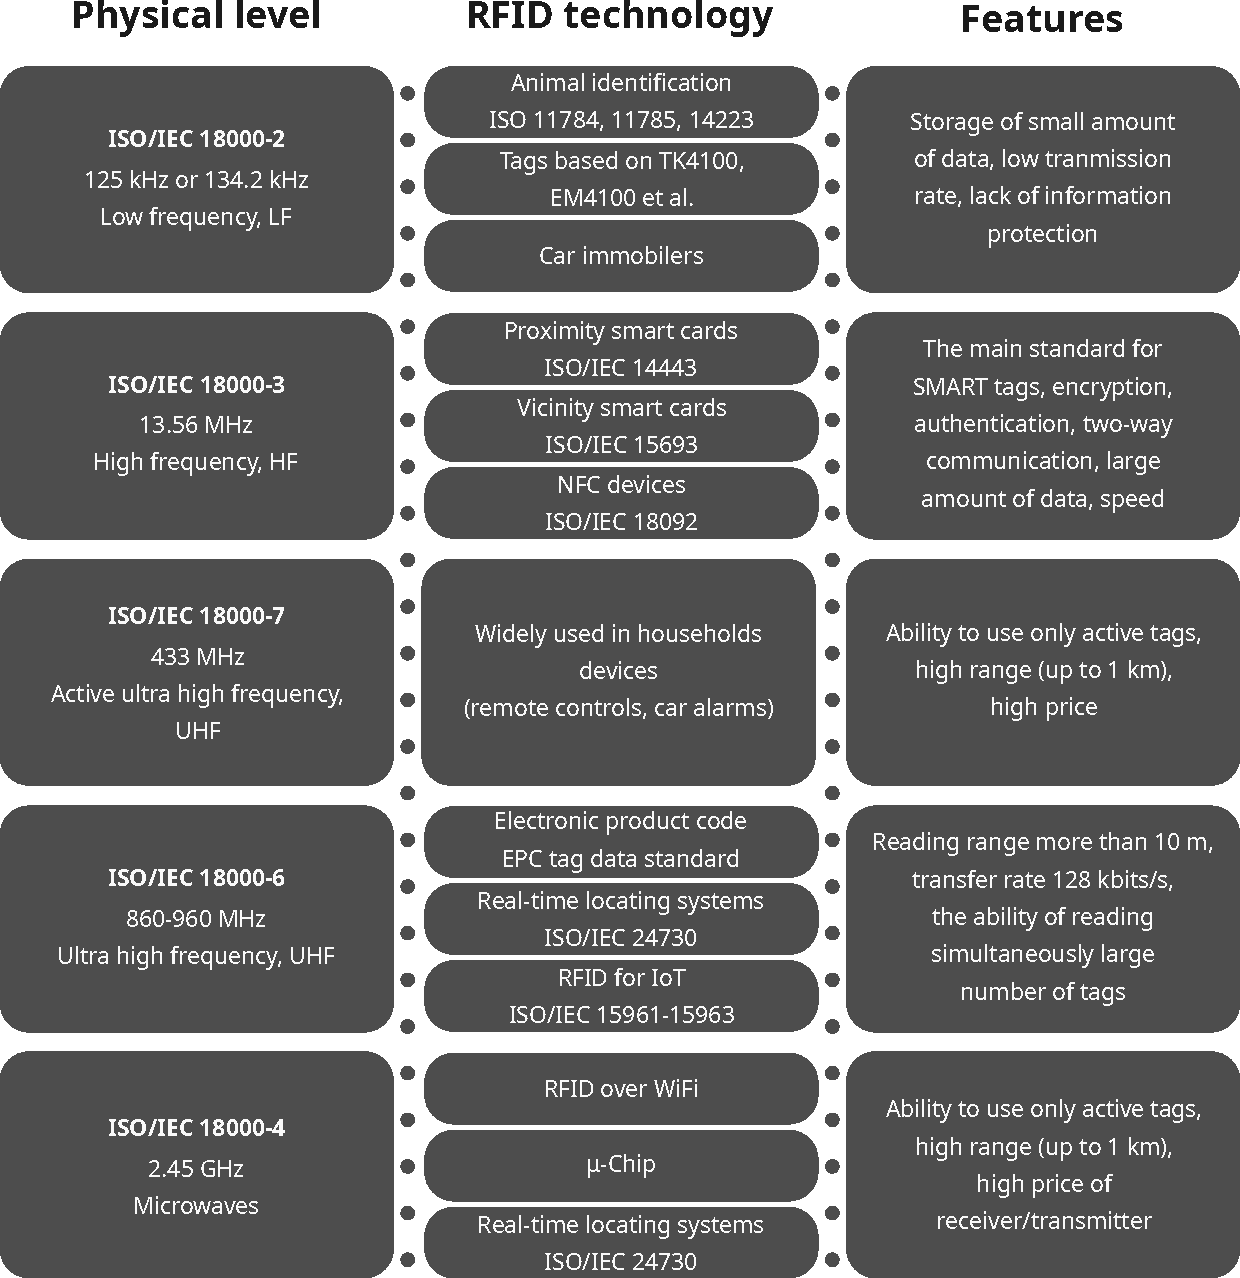
\includegraphics[width=14cm]{text/rfid_graph.pdf} % or example.eps, depending on the format you converted to
  \caption[RFID technology, standards and equipment.]{~RFID technology, standards and equipment. Taken from~\cite{masyuk2019information}, redrawn by the author.}
  \label{fig:rfid-graph}
\end{figure}


\section{Magic Cards}

In most cases, tags have some part of their data unwritable, given by the manufacturer. This part of the data may include, for example, the tag UID, which is therefore immutable. In the case of Mifare Classic 1k, the UID has been managed between manufacturers to ensure that no two cards have the same UID. By the time the security of the Mifare Classic tag had been breached, "compatible chipsets", or in other words "magic chipsets", had started to be produced in China, which were capable of, among other things, forging the UID. These magic tags underwent a short evolution, became more stable and could emulate more types of cards. Later, the so-called "Ultimate Magic Card", also known as "Gen 4", was released, a tag that could emulate NTAG, Mifare Classic and Mifare Ultralight tags and all their variants.  It also supports complete control over ATQA, SAK, ATS values, UIDs, as well as UID length, supporting 4, 7 and 10 byte UIDs. There are plenty of other magic tags on the market that support different chipsets and offer different functionalities.~\cite{magiccards}


\section{Types of Tags and Their Characteristics}

The content of this section is a summary of information about types of tags that are later used in the practical part of the thesis. The tag types mentioned are some of those tags that can be emulated or cloned in some way. Their properties and, if they exist, their vulnerabilities are discussed.


\subsection{EM410x Tags}

EM410x tags are simple LF tags commonly used in plastic cards. EM410x is a set of individual tag subtypes, such as EM4100, EM4102, EM4105 which are manufactured by EM Microelectronics.~\cite{krumnikl2015em410x}

The tag itself contains a contactless transponder carrying only 8 bytes of read-only data and does not implement any encryption, making it quite simple. An unique code is assigned to each individual chip by laser fusing of poly silicon links.~\cite{krumnikl2015em410x}

The Figure~\ref{fig:em410xdata} shows the distribution of 64 bits in the tag memory. When the tag gets close to the RFID reader, it induces a voltage inside the tag and starts transmitting its 8 bytes of data, which it repeats as long as it has power~\cite{priority1designEM4100Protocol}.


\begin{figure}[h]
  \centering
  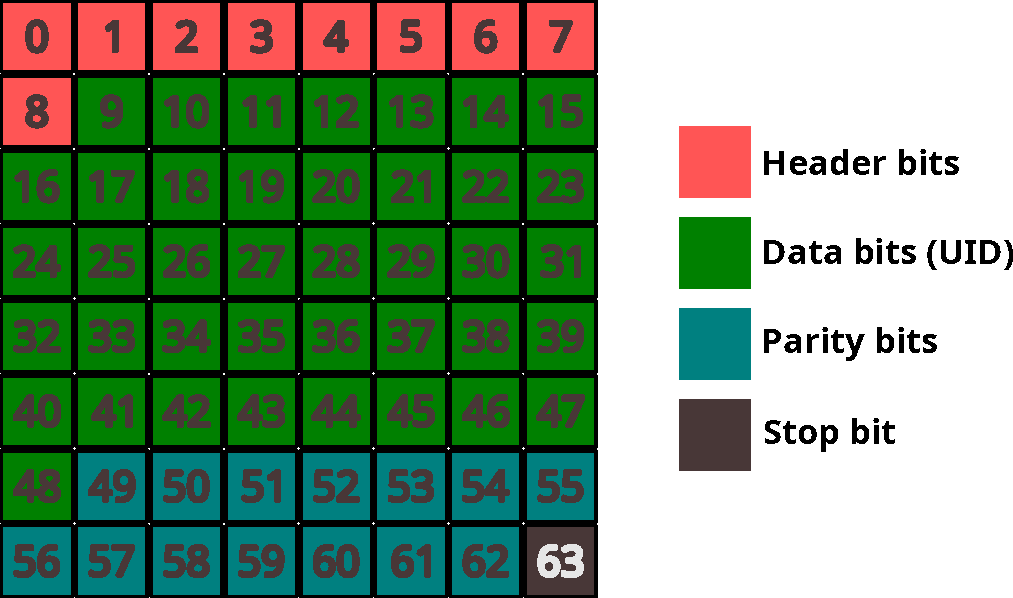
\includegraphics[width=9cm]{text/em410x_data.pdf} % or example.eps, depending on the format you converted to
  \caption[The memory organisation of EM410x tags.]{~The memory organisation of EM410x tags. Facts from~\cite{krumnikl2015em410x}, illustrated by the author.}
  \label{fig:em410xdata}
\end{figure}

As these tags does not employ any security features, the cloning process involves only copying the tag's ID and its associated data.~\cite{koscher2009EPC}

These tags contain different types of chips, e.g. chip EM. This particular chip is not capable of being written to. On the other hand, the T5577 chip is programmable and is capable of emulating various types of LF chips, such as the aforementioned EM chip, HID, or Indala.~\cite{lfchipsforum}


\subsection{Mifare Ultralight}

The simplest version of Ultralight tags, Mifare Ultralight, is an HF tag developed by NXP Semiconductors for use as a single or reusable ticket in transportation, as loyalty cards or day passes for events. The mechanical and electronic features are tailor-made to meet the requirements of paper ticket manufacturers. Mifare Ultralight adheres to the ISO/IEC 14443 A standard. The operating distance is up to 100 mm depending on antenna geometry and reader configuration.~\cite{ultralightdatasheet}

Mifare implements an intelligent anticollision algorithm which enables simultaneous multicard operation. The algorithm individually selects each card based on the tag UID and ensures that every transaction is correctly executed.~\cite{ultralightdatasheet}

The security of the card lies in the following measures:

\begin{itemize}
    \item  7-byte UID in accordance with ISO/IEC 14443-3 standard,
    \item 32-bit user definable OTP area (One-Time Programmable area), and
    \item read-only locking function per page.
\end{itemize}
The cloning process of the Mifare Ultralight card is trivial, because the tag does not implement any encryption. It is only necessary to copy the contents of the EEPROM memory to another tag, or even change the UID (if the target tag is a magic tag).~\cite{ultralightdatasheet, preucil2023surveying}

The EEPROM 512-bit memory is organised into 16 pages with 4 bytes per page, as ilustrated in Figure~\ref{fig:ultralightmemory}.~\cite{ultralightdatasheet}

\begin{figure}[ht]
  \centering
  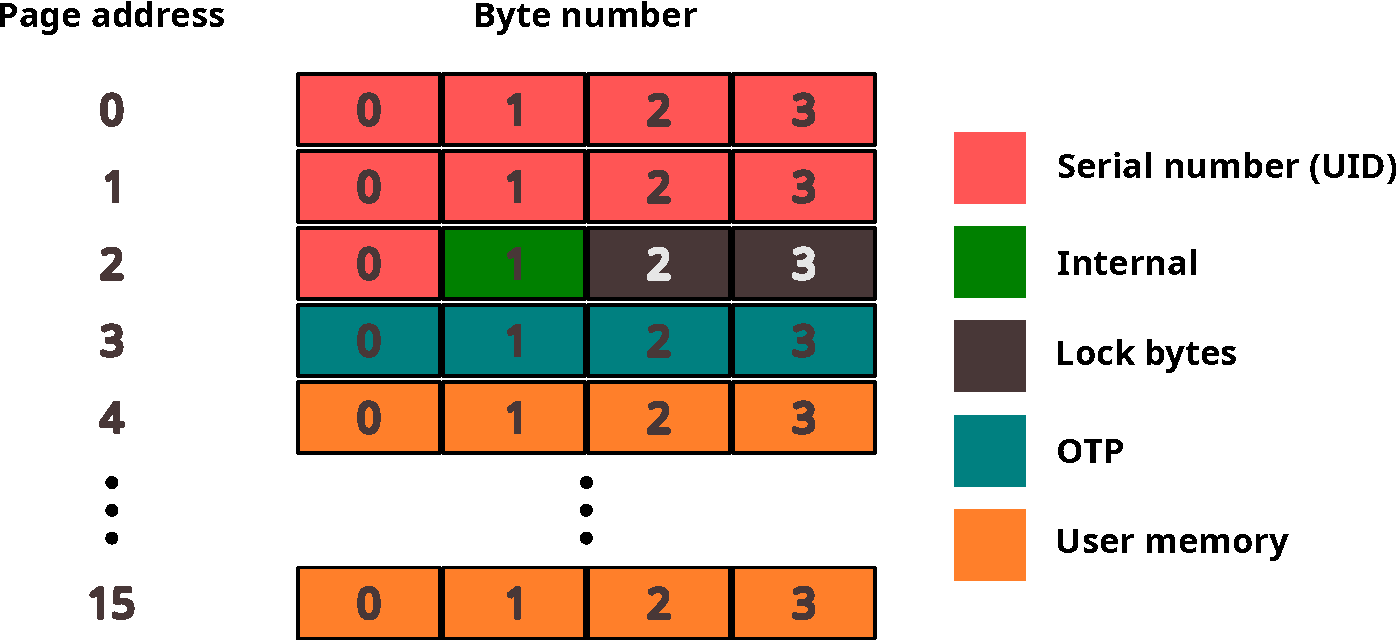
\includegraphics[width=12cm]{text/ultralight_data.pdf}
  \caption[The memory organisation of Mifare Ultralight tags.]{~The memory organisation of Mifare Ultralight tags. Facts from~\cite{ultralightdatasheet}, illustrated by the author.}
  \label{fig:ultralightmemory}
\end{figure}

A slightly more complex version of this tag, the Mifare Ultralight EV1, uses password protection. In its configuration, it holds the page number from which all pages are password protected. The EV1 therefore does not need to have any secured pages, so it is backwards compatible with the basic version of Mifare Ultralight. Secured Mifare Ultralight EV1 pages can be read after sniffing the trafic between the card and the reader, without sniffing it is possible to read and clone only the non-secure ones.~\cite{ultralightev1datasheet, preucil2023surveying}

\subsection{Mifare Classic}

Mifare Classic tags are HF tags also manufactured by NXP Semiconductors, used in public transportation, as school or campus tags, or in car parking. Mifare Classic tags are available in 1k and 4k versions. Like Mifare Ultralight, Mifare Classic tags implement an intelligent anticollision function. It is also in compliance with ISO/IEC 14443 A standard. The tag memory is divided into data blocks of 16 bytes. The Mifare Classic 1k contains 16 sectors of 4 blocks and the larger Mifare Classic 4k memory contains the first 32 sectors of 4 blocks and the remaining 8 sectors of 16 blocks, making it backwards compatible with 1k version. A schematic of the Mifare Classic 1k memory can be seen in Figure~\ref{fig:classsic1kmemory}.~\cite{classic1kdatasheet, classic4kdatasheet}

\begin{figure}[ht]
  \centering
  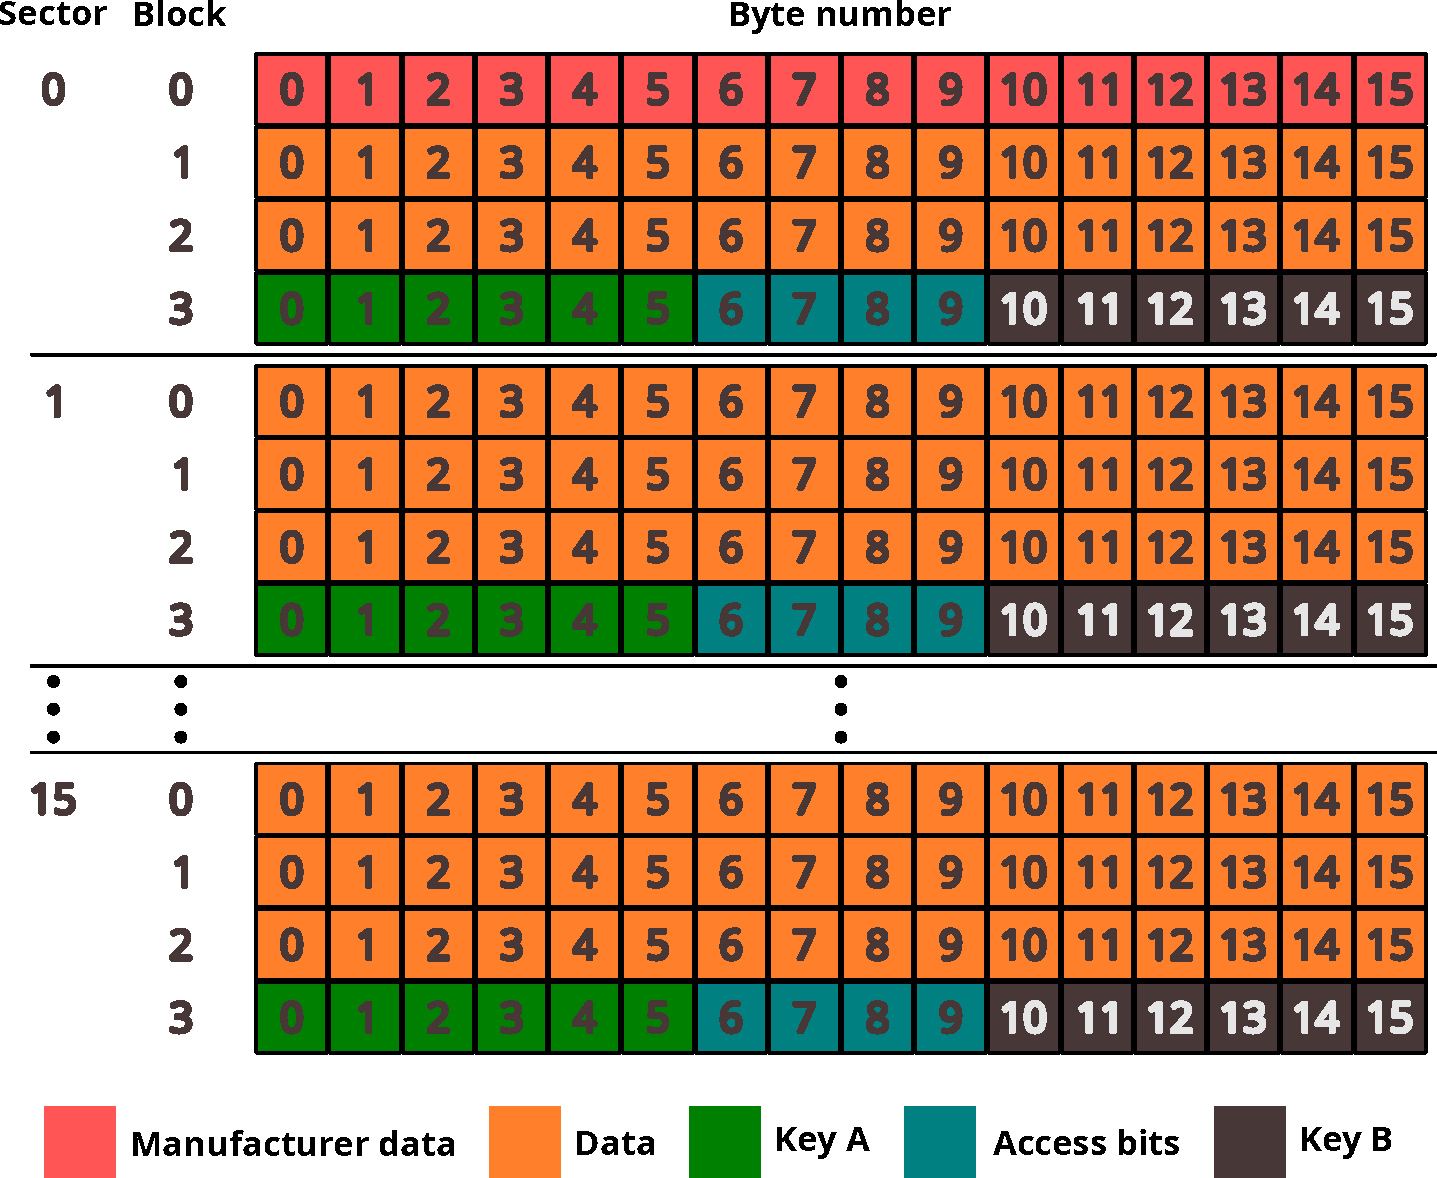
\includegraphics[width=12cm]{text/classic1k_data.pdf}
  \caption[The memory organisation of Mifare Classic 1k tags.]{~The memory organisation of Mifare Classic 1k tags. Facts from~\cite{classic1kdatasheet}, illustrated by the author.}
  \label{fig:classsic1kmemory}
\end{figure}

The first 4 bytes of block 0 of sector zero contain the tag UID. The fifth byte contains the BCC value, which is calculated by successive XORing of all UID bytes. The remaining 11 bytes of sector zero are manufacturer data.~\cite{gans2008practical}

At the end of each sector is a block containing keys A and B, which are used for authentication, the access conditions define the operations that can be performed in this sector. This block has special properties. Key A is not readable and Key B can be set to be readable. The reader must authenticate for a sector before any memory operations are allowed.~\cite{gans2008practical}

The communication encrypted using the stream cipher CRYPTO1 was reverse engineered. The authentication proceeds as follows:

\begin{enumerate}
    \item The tag is selected in the anticollision phase and sends its UID to the reader.
    \item The reader asks for authentication of a specific block.
    \item The tag sends a challenge nonce \( n_{T} \).
    \item The reader responds with its own encrypted challenge nonce \( n_{R} \) and with the response\\
    \(
        a_{R} = \text{suc}^{64}(n_{T})
    \) where

    \begin{equation*}
        suc(x_0 x_1 \ldots x_{31}) := x_1 x_2 \ldots x_{31} L_{16}(x_{16} x_{17} \ldots x_{31})
    \end{equation*}


    and

    \begin{equation*}
        L_{16}(x_0x_1 \ldots x_{15}) := x_0 \oplus x_2 \oplus x_3 \oplus x_5
    \end{equation*}.


\item Authentication is concluded by the tag response \( a_{T} = \text{suc}^{96}(n_{R}) \).~\cite{tezcan2017brute}
\end{enumerate}

 There are several known vulnerabilities in Mifare Classic, such as short key lengths, predictable nonces or nested authentication. You can read more about them in~\cite{meijer2015mifare}.


\subsection{Legic Prime}

Legic Prime is a HF tag developed by Legic. It was launched in 1992 and used in acceess control, but has also found use in payment applications. It can hold several applications, however this is rarely ever seen. There are 3 variants:

\begin{itemize}
    \item MIM22, which is outdated,
    \item MIM256, which has a memory of 234 bytes, and
    \item MIM1024, with a memory of 1002 bytes.
\end{itemize}
Legic takes obscurity to the extreme, there is no official documentation beyond layer 1+2, and compared to Mifare Classic it is much more challenging to get tags and readers on the free market.~\cite{nohllegic}

It uses its proprietary radio protocol and "legic encryption". The security systems breaks in two places, where cryptography is missing:

\begin{enumerate}
    \item both cards and readers do not hold secret keys and cannot authenticate each other, allowing an attacker to assume either role and read, write or spoof cards and readers, and
    \item the lack of cryptography allows attacks against Legic's trust delegation model, which places cards in a hierarchy where higher level cards can produce lower level cards. Since there is no secret information to distinguish higher from lower levels of authorisation, any level can be spoofed for any Legic installation in the world.
\end{enumerate}
For these reasons, the Legic Prime system is not suitable for access control systems in the long term.~\cite{srlabsLegicPrime}




\subsection{Mifare Desfire}

Mifare DESFire tags are HF tags considered one of the most advanced RFID technologies.  Its EV1, EV2 and EV3 generations are considered secure and no attack has been described yet. It uses 3DES or AES hardware cryptographic engine for encoding transmission data. It can be used in building access, transport, closed-loop e-payment schemes and others. It is compliant to all 4 levels of ISO/IEC 14443 A. Tags use 7 byte UIDs. Since this type of card is considered to be secure, there is no point in discussing the memory contents in this paper. However, for reference it is worth mentioning that it holds data in the form of files and applications.~\cite{desfiredatasheet, preucil2023surveying}
